% Options for packages loaded elsewhere
\PassOptionsToPackage{unicode}{hyperref}
\PassOptionsToPackage{hyphens}{url}
%
\documentclass[
]{book}
\usepackage{amsmath,amssymb}
\usepackage{lmodern}
\usepackage{setspace} % add line to default template
\setstretch{1.2}      % add line to default template
\usepackage{iftex}
\ifPDFTeX
  \usepackage[T1]{fontenc}
  \usepackage[utf8]{inputenc}
  \usepackage{textcomp} % provide euro and other symbols
\else % if luatex or xetex
  \usepackage{unicode-math}
  \defaultfontfeatures{Scale=MatchLowercase}
  \defaultfontfeatures[\rmfamily]{Ligatures=TeX,Scale=1}
\fi
% Use upquote if available, for straight quotes in verbatim environments
\IfFileExists{upquote.sty}{\usepackage{upquote}}{}
\IfFileExists{microtype.sty}{% use microtype if available
  \usepackage[]{microtype}
  \UseMicrotypeSet[protrusion]{basicmath} % disable protrusion for tt fonts
}{}
\makeatletter
\@ifundefined{KOMAClassName}{% if non-KOMA class
  \IfFileExists{parskip.sty}{%
    \usepackage{parskip}
  }{% else
    \setlength{\parindent}{0pt}
    \setlength{\parskip}{6pt plus 2pt minus 1pt}}
}{% if KOMA class
  \KOMAoptions{parskip=half}}
\makeatother
\usepackage{xcolor}
\IfFileExists{xurl.sty}{\usepackage{xurl}}{} % add URL line breaks if available
\IfFileExists{bookmark.sty}{\usepackage{bookmark}}{\usepackage{hyperref}}
\hypersetup{
  pdftitle={Statistical Analysis of Behavioral Data},
  pdfauthor={Ahmad Ehyaei; Sara Ershadmanesh},
  hidelinks,
  pdfcreator={LaTeX via pandoc}}
\urlstyle{same} % disable monospaced font for URLs
\usepackage{color}
\usepackage{fancyvrb}
\newcommand{\VerbBar}{|}
\newcommand{\VERB}{\Verb[commandchars=\\\{\}]}
\DefineVerbatimEnvironment{Highlighting}{Verbatim}{commandchars=\\\{\}}
% Add ',fontsize=\small' for more characters per line
\usepackage{framed}
\definecolor{shadecolor}{RGB}{248,248,248}
\newenvironment{Shaded}{\begin{snugshade}}{\end{snugshade}}
\newcommand{\AlertTok}[1]{\textcolor[rgb]{0.94,0.16,0.16}{#1}}
\newcommand{\AnnotationTok}[1]{\textcolor[rgb]{0.56,0.35,0.01}{\textbf{\textit{#1}}}}
\newcommand{\AttributeTok}[1]{\textcolor[rgb]{0.77,0.63,0.00}{#1}}
\newcommand{\BaseNTok}[1]{\textcolor[rgb]{0.00,0.00,0.81}{#1}}
\newcommand{\BuiltInTok}[1]{#1}
\newcommand{\CharTok}[1]{\textcolor[rgb]{0.31,0.60,0.02}{#1}}
\newcommand{\CommentTok}[1]{\textcolor[rgb]{0.56,0.35,0.01}{\textit{#1}}}
\newcommand{\CommentVarTok}[1]{\textcolor[rgb]{0.56,0.35,0.01}{\textbf{\textit{#1}}}}
\newcommand{\ConstantTok}[1]{\textcolor[rgb]{0.00,0.00,0.00}{#1}}
\newcommand{\ControlFlowTok}[1]{\textcolor[rgb]{0.13,0.29,0.53}{\textbf{#1}}}
\newcommand{\DataTypeTok}[1]{\textcolor[rgb]{0.13,0.29,0.53}{#1}}
\newcommand{\DecValTok}[1]{\textcolor[rgb]{0.00,0.00,0.81}{#1}}
\newcommand{\DocumentationTok}[1]{\textcolor[rgb]{0.56,0.35,0.01}{\textbf{\textit{#1}}}}
\newcommand{\ErrorTok}[1]{\textcolor[rgb]{0.64,0.00,0.00}{\textbf{#1}}}
\newcommand{\ExtensionTok}[1]{#1}
\newcommand{\FloatTok}[1]{\textcolor[rgb]{0.00,0.00,0.81}{#1}}
\newcommand{\FunctionTok}[1]{\textcolor[rgb]{0.00,0.00,0.00}{#1}}
\newcommand{\ImportTok}[1]{#1}
\newcommand{\InformationTok}[1]{\textcolor[rgb]{0.56,0.35,0.01}{\textbf{\textit{#1}}}}
\newcommand{\KeywordTok}[1]{\textcolor[rgb]{0.13,0.29,0.53}{\textbf{#1}}}
\newcommand{\NormalTok}[1]{#1}
\newcommand{\OperatorTok}[1]{\textcolor[rgb]{0.81,0.36,0.00}{\textbf{#1}}}
\newcommand{\OtherTok}[1]{\textcolor[rgb]{0.56,0.35,0.01}{#1}}
\newcommand{\PreprocessorTok}[1]{\textcolor[rgb]{0.56,0.35,0.01}{\textit{#1}}}
\newcommand{\RegionMarkerTok}[1]{#1}
\newcommand{\SpecialCharTok}[1]{\textcolor[rgb]{0.00,0.00,0.00}{#1}}
\newcommand{\SpecialStringTok}[1]{\textcolor[rgb]{0.31,0.60,0.02}{#1}}
\newcommand{\StringTok}[1]{\textcolor[rgb]{0.31,0.60,0.02}{#1}}
\newcommand{\VariableTok}[1]{\textcolor[rgb]{0.00,0.00,0.00}{#1}}
\newcommand{\VerbatimStringTok}[1]{\textcolor[rgb]{0.31,0.60,0.02}{#1}}
\newcommand{\WarningTok}[1]{\textcolor[rgb]{0.56,0.35,0.01}{\textbf{\textit{#1}}}}
\usepackage{longtable,booktabs,array}
\usepackage{calc} % for calculating minipage widths
% Correct order of tables after \paragraph or \subparagraph
\usepackage{etoolbox}
\makeatletter
\patchcmd\longtable{\par}{\if@noskipsec\mbox{}\fi\par}{}{}
\makeatother
% Allow footnotes in longtable head/foot
\IfFileExists{footnotehyper.sty}{\usepackage{footnotehyper}}{\usepackage{footnote}}
\makesavenoteenv{longtable}
\usepackage[normalem]{ulem}
% Avoid problems with \sout in headers with hyperref
\pdfstringdefDisableCommands{\renewcommand{\sout}{}}
\setlength{\emergencystretch}{3em} % prevent overfull lines
\providecommand{\tightlist}{%
  \setlength{\itemsep}{0pt}\setlength{\parskip}{0pt}}
\setcounter{secnumdepth}{5}

\usepackage{booktabs}
\usepackage{longtable}
\usepackage{array}
\usepackage{multirow}
\usepackage{wrapfig}
\usepackage{float}
\usepackage{colortbl}
\usepackage{pdflscape}
\usepackage{tabu}
\usepackage{threeparttable}
\usepackage{threeparttablex}
\usepackage[normalem]{ulem}
\usepackage{makecell}
\usepackage{xcolor}
\usepackage{amsmath}
\usepackage{caption}
\ifLuaTeX
  \usepackage{selnolig}  % disable illegal ligatures
\fi

\title{Statistical Analysis of Behavioral Data}
\author{Ahmad Ehyaei \and Sara Ershadmanesh}
\date{16 Oktober, 2021}

% ...................................................................... %
%
%               Add MPI Custom Template For Long Reprt
%
% ...................................................................... %
\usepackage{float}

% ...................................................................... %
% Load Packages
% tables requirement kableExtra packages2
% TODO: table striped dont work

% ...................................................................... %
% Add MPI Colors

% Colors extract from Max-Planck Society CD Manula
% https://docplayer.org/2328711-Max-planck-institut-das-erscheinungsbild-der-max-planck-gesellschaft-4-ueberarbeitete-auflage.html
\usepackage{xcolor}

\definecolor{MPIGreen}{HTML}{116656}
\definecolor{MPIGray}{HTML}{DDDED6}
\definecolor{MPIBlue}{HTML}{009EE2}
\definecolor{MPIRed}{HTML}{E90649}
\definecolor{MPILightBlue}{HTML}{40BDE8}
\definecolor{MPIOrange}{HTML}{FF7300}
\definecolor{MPIYellow}{HTML}{FFCE09}
\definecolor{MPIPink}{HTML}{FA9FCC}
\definecolor{MPILightGreen}{HTML}{62BD19}
\definecolor{MPILivingCoral}{HTML}{FC766A}
\definecolor{MPIPacificCoast}{HTML}{5B84B1}

% set titlepage top, bottom, text and rule color

\definecolor{titlepageTopColor}{HTML}{f03e4c}


\definecolor{titlepageBottomColor}{HTML}{009EE2}


\definecolor{titlepageTextColor}{HTML}{FFFFFF}

\definecolor{titlepageAuthorTextColor}{HTML}{f03e4c}


\definecolor{titlePageColor}{HTML}{009EE2}

\definecolor{titlePageRuleColor}{HTML}{ffffff}

\definecolor{pageBackgroundColor}{HTML}{f6f6f6}

\definecolor{bannerColor}{HTML}{40BDE8}

\definecolor{bannerTextColor}{HTML}{000000}

\definecolor{chapterTitleColor}{HTML}{E90649}

% Set Initial Values

\def\titlepageRuleHeight{10}


\def\titleVjust{250}

\def\titleHjust{30}


\def\authorVjust{80}

\def\authorHjust{30}


% end of color and value definition
%......................................................................%

%......................................................................%
% set default hold position of figure and table
\makeatletter
  \providecommand*\setfloatlocations[2]{\@namedef{fps@#1}{#2}}
\makeatother
\setfloatlocations{figure}{H}
\setfloatlocations{table}{H}
%......................................................................%


%......................................................................%
% Add Main Fonts

\usepackage{fontspec}
% set main font univers
\setmainfont[ Path = src/fonts/]{Univers-light-normal.ttf}[
BoldFont = UniversBlack.ttf,
ItalicFont = UniversLTStd.otf,
BoldItalicFont = UniversLTStd-Bold.otf
]
% define Bodoni font for title
\newfontfamily\Bodoni[
  Path=src/fonts/,
  LetterSpace=2.0,
  WordSpace={10,0,0},
  HyphenChar=None,
  PunctuationSpace=WordSpace
  ]{BodoniFLF-Roman.ttf}
% \newfontfamily\BodoniBold[Path=src/fonts/]{BodoniFLF-Bold.ttf}
% \newfontfamily\BodoniBoldItalic[Path=src/fonts/]{BodoniFLF-BoldItalic.ttf}
% \newfontfamily\BodoniItalic[Path=src/fonts/]{BodoniFLF-Italic.ttf}


%......................................................................%
% add colored box environments

\usepackage[most]{tcolorbox}
\usepackage{awesomebox}

\newtcolorbox{info-box}{colback=cyan!5!white,arc=0pt,outer arc=0pt,colframe=cyan!60!black}
\newtcolorbox{warning-box}{colback=orange!5!white,arc=0pt,outer arc=0pt,colframe=orange!80!black}
\newtcolorbox{error-box}{colback=red!5!white,arc=0pt,outer arc=0pt,colframe=red!75!black}


% Think
\newenvironment{rmdThink}{
	\vspace*{0.5\baselineskip}
    \par\noindent
    \begin{tcolorbox}[enhanced, title={\textbf{\color{white}Think}},colback=MPIGreen!10!white, colframe=MPIGreen]
    \itshape
}{
    \end{tcolorbox}
    \par\ignorespacesafterend
}
\newtcolorbox{rmdthink}{colback=MPIGreen!10!white,colframe=MPIGreen,coltext=black,leftrule= 2mm,rightrule=0.5mm,bottomrule=0.5mm,toprule=0.5mm, boxsep=0.5pt,arc=2pt}

% Note
\newenvironment{rmdNote}{
	\vspace*{0.5\baselineskip}
    \par\noindent
    \begin{tcolorbox}[enhanced, title={\textbf{\color{white}Note}},colback=MPIRed!10!white, colframe=MPIRed]
    \itshape
}{
    \end{tcolorbox}
    \par\ignorespacesafterend
}
\newtcolorbox{rmdnote}{colback=MPIRed!10!white,colframe=MPIRed,coltext=black,leftrule= 2mm,rightrule=0.5mm,bottomrule=0.5mm,toprule=0.5mm, boxsep=0.5pt,arc=2pt}

% Tip
\newenvironment{rmdTip}{
	\vspace*{0.5\baselineskip}
    \par\noindent
    \begin{tcolorbox}[enhanced, title={\textbf{\color{white}Tip}},colback=MPILightGreen!10!white, colframe=MPILightGreen]
    \itshape
}{
    \end{tcolorbox}
    \par\ignorespacesafterend
}
\newtcolorbox{rmdtip}{colback=MPILightGreen!10!white,colframe=MPILightGreen,coltext=black,leftrule= 2mm,rightrule=0.5mm,bottomrule=0.5mm,toprule=0.5mm, boxsep=0.5pt,arc=2pt}

% warning
\newenvironment{rmdWarning}{
	\vspace*{0.5\baselineskip}
    \par\noindent
    \begin{tcolorbox}[enhanced, title={\textbf{\color{white}Warning}},colback=MPIOrange!10!white, colframe=MPIOrange]
    \itshape
}{
    \end{tcolorbox}
    \par\ignorespacesafterend
}
\newtcolorbox{rmdwarning}{colback=MPIOrange!10!white,colframe=MPIOrange,coltext=black,leftrule= 2mm,rightrule=0.5mm,bottomrule=0.5mm,toprule=0.5mm, boxsep=0.5pt,arc=2pt}

% todo
\newenvironment{rmdTodo}{
	\vspace*{0.5\baselineskip}
    \par\noindent
    \begin{tcolorbox}[enhanced, title={\textbf{\color{white}To Do}},colback=MPIBlue!10!white, colframe=MPIBlue]
    \itshape
}{
    \end{tcolorbox}
    \par\ignorespacesafterend
}
\newtcolorbox{rmdtodo}{colback=MPIBlue!10!white,colframe=MPIBlue,coltext=black,leftrule= 2mm,rightrule=0.5mm,bottomrule=0.5mm,toprule=0.5mm, boxsep=0.5pt,arc=2pt}



\newtcbtheorem[auto counter,number within=section]{Theorem}{Theorem}{%
                lower separated=false,fonttitle=\bfseries,
                colback=MPIGreen!10!white,colframe=MPIGreen,
                colbacktitle=MPIGreen, coltitle=white,
                enhanced,attach boxed title to top left={xshift=0.5cm,yshift=-2mm}
                }{thm}

\newtcbtheorem[auto counter,number within=section]{Definition}{Definition}{%
                lower separated=false,fonttitle=\bfseries,
                colback=MPILightGreen!10!white,colframe=MPILightGreen,
                colbacktitle=MPILightGreen, coltitle=white,
                enhanced,attach boxed title to top left={xshift=0.5cm,yshift=-2mm}
                }{defn}

\newtcbtheorem[auto counter,number within=section]{Lemma}{Lemma}{%
                lower separated=false,fonttitle=\bfseries,
                colback=MPILightBlue!10!white,colframe=MPILightBlue,
                colbacktitle=MPILightBlue, coltitle=white,
                enhanced,attach boxed title to top left={xshift=0.5cm,yshift=-2mm}
                }{lem}

\newtcbtheorem[auto counter,number within=section]{Corollary}{Corollary}{%
                lower separated=false,fonttitle=\bfseries,
                colback=MPIBlue!10!white,colframe=MPIBlue,
                colbacktitle=MPIBlue, coltitle=white,
                enhanced,attach boxed title to top left={xshift=0.5cm,yshift=-2mm}
                }{cor}

\newtcbtheorem[auto counter,number within=section]{Proposition}{Proposition}{%
                lower separated=false,fonttitle=\bfseries,
                colback=MPIYellow!10!white,colframe=MPIYellow,
                colbacktitle=MPIYellow, coltitle=white,
                enhanced,attach boxed title to top left={xshift=0.5cm,yshift=-2mm}
                }{prop}

\newtcbtheorem[auto counter,number within=section]{Exercise}{Exercise}{%
                lower separated=false,fonttitle=\bfseries,
                colback=MPIRed!10!white,colframe=MPIRed,
                colbacktitle=MPIRed, coltitle=white,
                enhanced,attach boxed title to top left={xshift=0.5cm,yshift=-2mm}
                }{exer}

\newtcbtheorem[auto counter,number within=section]{Example}{Example}{%
                lower separated=false,fonttitle=\bfseries,
                colback=MPIOrange!10!white,colframe=MPIOrange,
                colbacktitle=MPIOrange, coltitle=white,
                enhanced,attach boxed title to top left={xshift=0.5cm,yshift=-2mm}
                }{exam}

\newtcbtheorem[auto counter,number within=section]{Remark}{Remark}{%
                lower separated=false,fonttitle=\bfseries,
                colback=MPIPink!10!white,colframe=MPIPink,
                colbacktitle=MPIPink, coltitle=white,
                enhanced,attach boxed title to top left={xshift=0.5cm,yshift=-2mm}
                }{rmk}


\newtcbtheorem[auto counter,number within=section]{Proof}{Proof}{%
                lower separated=false,fonttitle=\bfseries,
                colback=MPILivingCoral!10!white,colframe=MPILivingCoral,
                colbacktitle=MPILivingCoral, coltitle=white,
                enhanced,attach boxed title to top left={xshift=0.5cm,yshift=-2mm}
                }{pr}

\newtcbtheorem[auto counter,number within=section]{Solution}{Solution}{%
                lower separated=false,fonttitle=\bfseries,
                colback=MPIPacificCoast!10!white,colframe=MPIPacificCoast,
                colbacktitle=MPIPacificCoast, coltitle=white,
                enhanced,attach boxed title to top left={xshift=0.5cm,yshift=-2mm}
                }{sol}


\newenvironment{rmdexer}{
    \par\noindent
    \textbf{\color{MPIRed}Exercise} \itshape
}{\par}

\newenvironment{rmdsol}{
    \par\noindent
    \textbf{\color{MPIPacificCoast}Solution} \itshape
}{\par}


%......................................................................%
% add packages for title page

\definecolor{rcolor}{HTML}{2165B6}
\definecolor{rconsole}{HTML}{7E7E7E}

\newtcolorbox{rmdconsole}{
  enhanced,
  boxrule=0pt,frame hidden,
  borderline west={4pt}{0pt}{rconsole},
  colback=rconsole!5!white,
  sharp corners
  }
\newtcolorbox{rmdcode}{
  enhanced,
  boxrule=0pt,frame hidden,
  borderline west={4pt}{0pt}{rcolor},
  colback=rcolor!5!white,
  sharp corners
  }

\BeforeBeginEnvironment{verbatim}{\begin{rmdconsole}}
\AfterEndEnvironment{verbatim}{\end{rmdconsole}}

\BeforeBeginEnvironment{Highlighting}{\begin{rmdcode}}
\AfterEndEnvironment{Highlighting}{\end{rmdcode}}
\definecolor{shadecolor}{HTML}{ffffff}

%......................................................................%
% add packages for title page

\usepackage{tikz}

\usepackage[margin=1.5cm,includehead=true,includefoot=true,centering]{geometry}

% ----------------------------------------------------------------------------- %
%                                   Set Geometry                                %
% ----------------------------------------------------------------------------- %

\makeatletter
\def\parsecomma#1,#2\endparsecomma{\def\page@x{#1}\def\page@y{#2}}
\tikzdeclarecoordinatesystem{page}{
    \parsecomma#1\endparsecomma
    \pgfpointanchor{current page}{north east}
    % Save the upper right corner
    \pgf@xc=\pgf@x%
    \pgf@yc=\pgf@y%
    % save the lower left corner
    \pgfpointanchor{current page}{south west}
    \pgf@xb=\pgf@x%
    \pgf@yb=\pgf@y%
    % Transform to the correct placement
    \pgfmathparse{(\pgf@xc-\pgf@xb)/2.*\page@x+(\pgf@xc+\pgf@xb)/2.}
    \expandafter\pgf@x\expandafter=\pgfmathresult pt
    \pgfmathparse{(\pgf@yc-\pgf@yb)/2.*\page@y+(\pgf@yc+\pgf@yb)/2.}
    \expandafter\pgf@y\expandafter=\pgfmathresult pt
}
\makeatother


% ---------------------------------------------------------------------------- %
% header and footer
% ---------------------------------------------------------------------------- %

\usepackage{fancyhdr}
\pagestyle{fancy}
\fancyhf{}
\fancyhead[R]{\leftmark}
\fancyfoot[R]{\thepage}
\renewcommand{\headrulewidth}{0.5pt}
% \renewcommand{\footrulewidth}{0.25pt}


% TODO: Add header and footer options
% \lhead{}
% \chead{}
% \rhead{}
% \lfoot{}
% \cfoot{}
% \rfoot{}


% ---------------------------------------------------------------------------- %
% Banner Page Header and Footer Style



% ---------------------------------------------------------------------------- %
% Add Page Background


% ---------------------------------------------------------------------------- %
% Add Page Background Color

\usepackage{eso-pic}
\newcommand\BackPage{%
\begin{tikzpicture}[remember picture,overlay]
\fill[pageBackgroundColor](current page.south west) rectangle (\paperwidth,\paperheight);
\end{tikzpicture}%
}

%......................................................................%
% Remove Blank Page after Table of Contents and between chapter


%----------------------------------------------------------------------------------------
% Chapter Design
\usepackage{titlesec}

\titleformat{\section}[block]
  {\huge\color{chapterTitleColor}}
  {\filright \textbf{\thesection}\vspace{1ex}}{12pt}
  {}
  [\titlerule]

\titleformat{\subsection}[block]
  {\Large\color{chapterTitleColor}}
  {\filright \textbf{\thesubsection}\vspace{1ex}}{12pt}
  {}
  []



%----------------------------------------------------------------------------------------
% Remove page number in toc and strange white first page

%......................................................................%
%
%               End of Modifications
%
%......................................................................%


\begin{document}
%......................................................................%
%               Add Titlepage
%......................................................................%


\begin{titlepage}

%......................................................................%
%                         Max-Planck Society Design

\begin{tikzpicture}[remember picture,overlay]



% add title page top color
\fill[titlepageTopColor] (page cs:-1,0.25) rectangle (current page.north east);



% add white rule


\node[inner sep=0pt] at (page cs:0,-0.38){\includegraphics[width=\paperwidth]{src/img/bottom\_background.png}};

%......................................................................%


%......................................................................%
%                         FullCover Color Page Design

%......................................................................%




% add main logo % TODO: add else
\node[inner sep=0pt] at (page cs:0.672,0.795){
\includegraphics[height=0.126\paperheight]{src/icon/MPILogoWhite.eps}};
% add secondary logo % TODO: add else
\node[inner sep=0pt] at (page cs:0.672,-0.795){};

% add title and subtitle
% TODO: use bodoni font in title
% \node[below,text width=\paperwidth,font=\color{titlepageTextColor}] at (page cs:0.15+\titleHjust,0.57+\titleVjust) {
\node[below,text width=\paperwidth,font=\color{titlepageTextColor}] at (page cs:0.0+\titleHjust,0.0+\titleVjust) {

    \Huge{\uppercase{Statistical Analysis of Behavioral Data}}
  \vspace{0.3cm}
  
  
  % add bodoni font to date
    \huge{\uppercase{16 Oktober, 2021}}
  \vspace{0.3cm}
  
  \vspace{0.6cm}
    \Large{ Max Planck Institute for Biological Cybernetics}
  \vspace{0.1cm}
  
    \large{Tübingen}
  };

\node[below,text width=\paperwidth,font=\color{titlepageTextColor}] at (page cs:0.0+\authorHjust,0.0+\authorVjust) {
    \huge{\textsf{\textcolor{titlepageAuthorTextColor}{Ahmad Ehyaei}\textcolor{titlepageAuthorTextColor}{,} \textcolor{titlepageAuthorTextColor}{Sara Ershadmanesh}}}
  \vspace{0.3cm}
  };

\end{tikzpicture}
\end{titlepage}
% \restoregeometry

% end design titlepage
%......................................................................%

%......................................................................%
% Add Page Background

\ClearShipoutPicture
\AddToShipoutPicture{\BackPage}


% add these lines for simple report template
% end add



% add from eisvogel template




% Add Table of Contents
{
\setcounter{tocdepth}{4}
\tableofcontents
}




\frontmatter

\mainmatter

\hypertarget{introduction}{%
\chapter{Introduction}\label{introduction}}

The bookdown framwrok is a free R package that makes it easier to write books and long reports using R Markdown. PDF, Gitbook, and epub are some of bookdown's output formats.

\hypertarget{markdown}{%
\chapter{Markdown}\label{markdown}}

Markdown is a basic syntax that allows you to format text using headers, lists, boldface, and other formatting options. This markup language is widely used, and you'll almost certainly find apps that support it. Here's a brief rundown of what Markdown syntax is, how to use it.

\hypertarget{headers}{%
\section{Headers}\label{headers}}

\begin{verbatim}
#    heading 1 
##   heading 2 
###  heading 3 
#### heading 4
#####  heading 5 
###### heading 6
\end{verbatim}

\hypertarget{emphasis}{%
\section{Emphasis}\label{emphasis}}

\begin{verbatim}
_Emphasized text_ or *Emphasized text*

~~Strikethrough text~~

__Strong text__ or **Strong text**

Strikethrough uses two tildes. ~~Scratch this.~~

___Strong emphasized text___ or ***Strong emphasized text***
\end{verbatim}

\emph{Emphasized text} or \emph{Emphasized text}

\sout{Strikethrough text}

\textbf{Strong text} or \textbf{Strong text}

Strikethrough uses two tildes. \sout{Scratch this.}

\textbf{\emph{Strong emphasized text}} or \textbf{\emph{Strong emphasized text}}

\hypertarget{links}{%
\section{Links}\label{links}}

\begin{verbatim}
[My GitHub Repository](https://github.com/Ehyaei) or https://github.com/Ehyaei

[heading-1](#heading-1 "Goto heading-1")
\end{verbatim}

\href{https://github.com/Ehyaei}{My GitHub Repository} or \url{https://github.com/Ehyaei}

\protect\hyperlink{Emphasis}{Emphasis}

\hypertarget{blockquotes}{%
\section{Blockquotes}\label{blockquotes}}

\begin{verbatim}
> To be, or not to be, that is the question.

>> To be, or not to be, that is the question.
\end{verbatim}

\begin{quote}
To be, or not to be, that is the question.
\end{quote}

\begin{quote}
\begin{quote}
To be, or not to be, that is the question.
\end{quote}
\end{quote}

\hypertarget{lists}{%
\section{Lists}\label{lists}}

\begin{Shaded}
\begin{Highlighting}[]
\NormalTok{* unordered list }
\NormalTok{* item 2\textasciigrave{}  }
\NormalTok{     + sub{-}item 1  }
\NormalTok{     + sub{-}item 2  }

\NormalTok{1. ordered list\textasciigrave{}  }
\NormalTok{2. item 2\textasciigrave{}  }
\NormalTok{     + sub{-}item 1  }
\NormalTok{     + sub{-}item 2  }
\end{Highlighting}
\end{Shaded}

\begin{itemize}
\tightlist
\item
  unordered list
\item
  item 2

  \begin{itemize}
  \tightlist
  \item
    sub-item 1
  \item
    sub-item 2
  \end{itemize}
\end{itemize}

\begin{enumerate}
\def\labelenumi{\arabic{enumi}.}
\tightlist
\item
  ordered list
\item
  item 2

  \begin{itemize}
  \tightlist
  \item
    sub-item 1
  \item
    sub-item 2
  \end{itemize}
\end{enumerate}

\hypertarget{task-list}{%
\section{Task List}\label{task-list}}

\begin{verbatim}
- [x] task 1
- [ ] task 2 

- [ ] task 1
  - [ ] subtask
\end{verbatim}

\begin{itemize}
\item[$\boxtimes$]
  task 1
\item[$\square$]
  task 2
\item[$\square$]
  task 1

  \begin{itemize}
  \tightlist
  \item[$\square$]
    subtask
  \end{itemize}
\end{itemize}

\hypertarget{table}{%
\section{Table}\label{table}}

\begin{verbatim}
Header1 | Header2
------ | ------
Cell11 | Cell12
Cell21 | Cell22 
\end{verbatim}

\begin{longtable}[]{@{}ll@{}}
\toprule
Header1 & Header2 \\
\midrule
\endhead
Cell11 & Cell12 \\
Cell21 & Cell22 \\
\bottomrule
\end{longtable}

\hypertarget{code-and-formula}{%
\chapter{Code and Formula}\label{code-and-formula}}

We can simply execute R codes among text in chunk contexts using RMakrdown. There are several possibilities in each chunk. Set \texttt{echo=TRUE}, for example, if you want to show the code.

\begin{Shaded}
\begin{Highlighting}[]
\FunctionTok{summary}\NormalTok{(cars)}
\NormalTok{     speed           dist       }
\NormalTok{ Min.   }\SpecialCharTok{:} \FloatTok{4.0}\NormalTok{   Min.   }\SpecialCharTok{:}  \FloatTok{2.00}  
\NormalTok{ 1st Qu.}\SpecialCharTok{:}\FloatTok{12.0}\NormalTok{   1st Qu.}\SpecialCharTok{:} \FloatTok{26.00}  
\NormalTok{ Median }\SpecialCharTok{:}\FloatTok{15.0}\NormalTok{   Median }\SpecialCharTok{:} \FloatTok{36.00}  
\NormalTok{ Mean   }\SpecialCharTok{:}\FloatTok{15.4}\NormalTok{   Mean   }\SpecialCharTok{:} \FloatTok{42.98}  
\NormalTok{ 3rd Qu.}\SpecialCharTok{:}\FloatTok{19.0}\NormalTok{   3rd Qu.}\SpecialCharTok{:} \FloatTok{56.00}  
\NormalTok{ Max.   }\SpecialCharTok{:}\FloatTok{25.0}\NormalTok{   Max.   }\SpecialCharTok{:}\FloatTok{120.00}  
\end{Highlighting}
\end{Shaded}

We can run inline R code \texttt{2\^{}10=} 1024

\hypertarget{math-formula}{%
\section{Math Formula}\label{math-formula}}

We can easily write math expressions by latex syntax.
Inline LateX equations can be written in a pair of dollar signs

\[f\left(k\right)=\binom{n}{k}p^k\left(1-p\right)^{n-k}\]
Also, we can write formulas by using dollar signs. For example, if we write \texttt{\$\textbackslash{}beta\$} then we see \(\beta\).

\hypertarget{figure}{%
\chapter{Figure}\label{figure}}

This package includes several ggplot themes and palettes for creating plots with
MPI custom design.

\hypertarget{color-palette}{%
\section{Color Palette}\label{color-palette}}

To find a color palette, Some colors are chosen from the Pantone list that is different from the two main colors. Color selection is a process in progress.

\begin{Shaded}
\begin{Highlighting}[]
\NormalTok{scales}\SpecialCharTok{::}\FunctionTok{show\_col}\NormalTok{(}\FunctionTok{palette\_mpi}\NormalTok{(),}\AttributeTok{ncol =} \DecValTok{3}\NormalTok{)}
\end{Highlighting}
\end{Shaded}

\begin{center}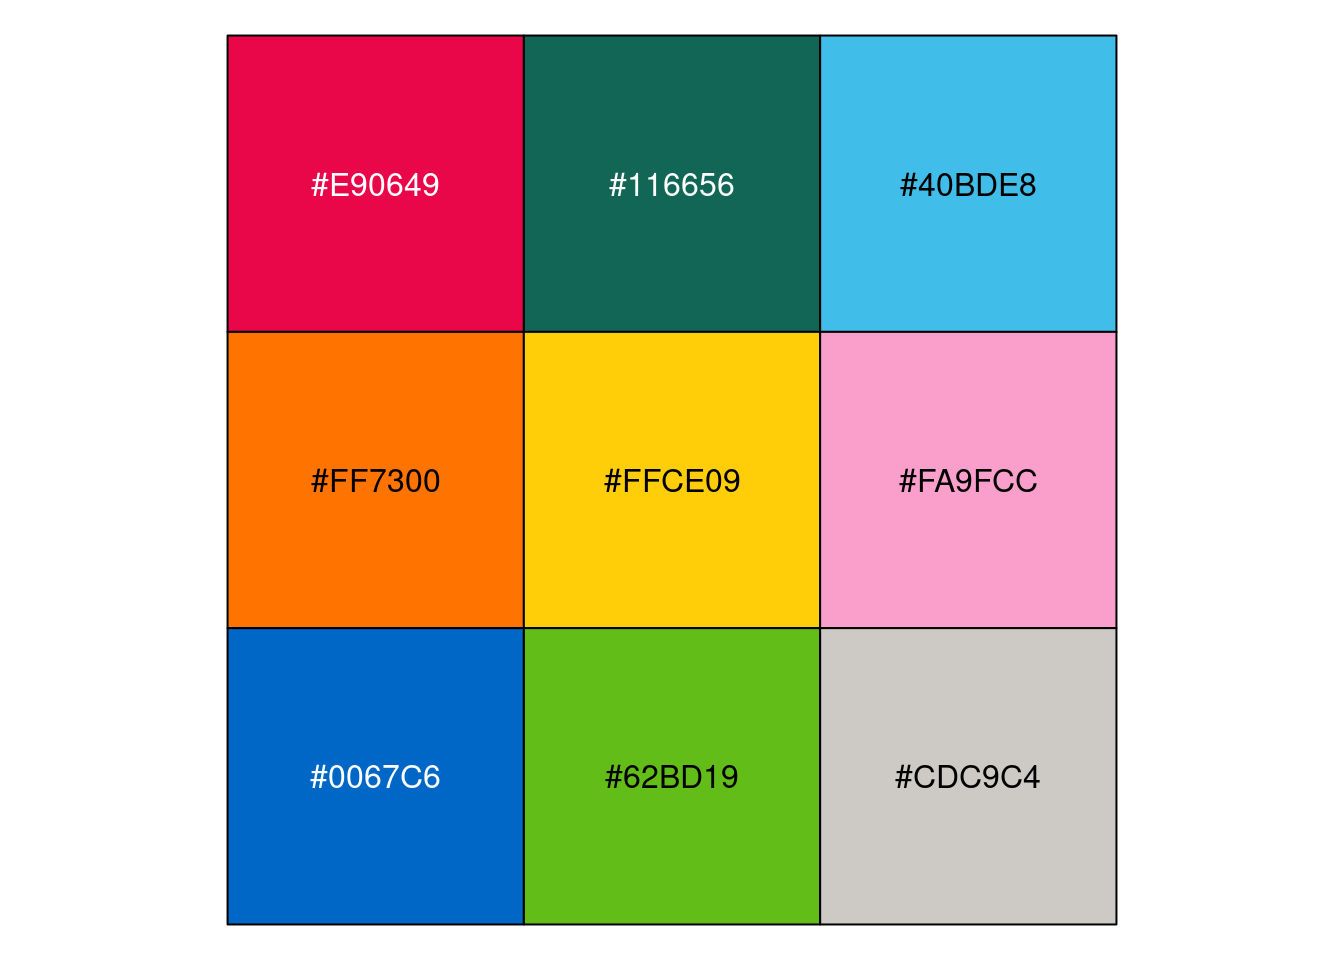
\includegraphics[width=0.5\linewidth]{figures/mpithemes_palette-1} \end{center}

There are some examples here,

\begin{center}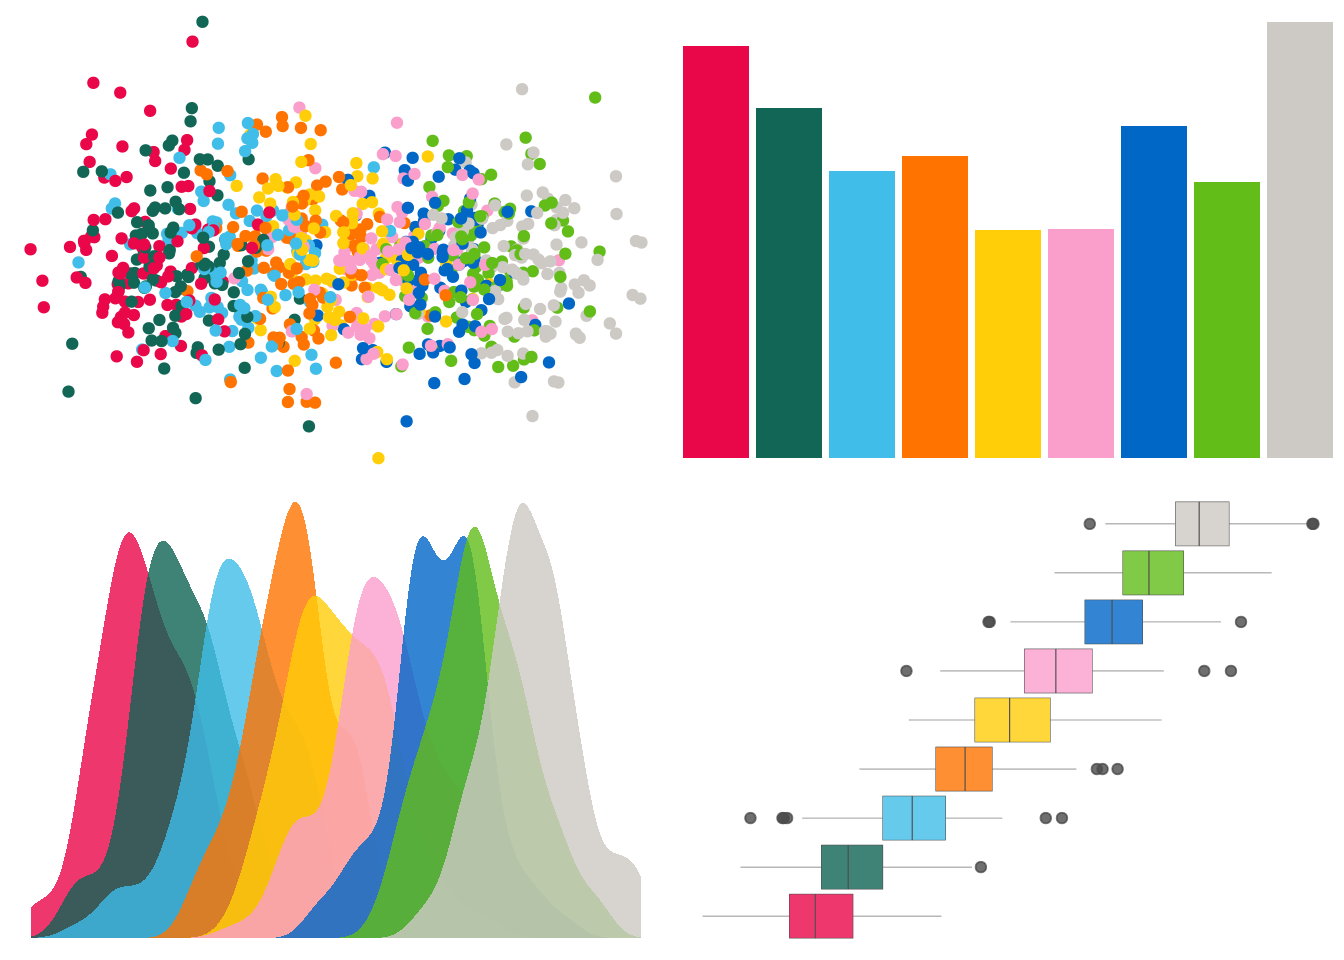
\includegraphics[width=1\linewidth]{figures/mpithemes_colors-1} \end{center}

A continuous palette can be seen in the example below.

\begin{center}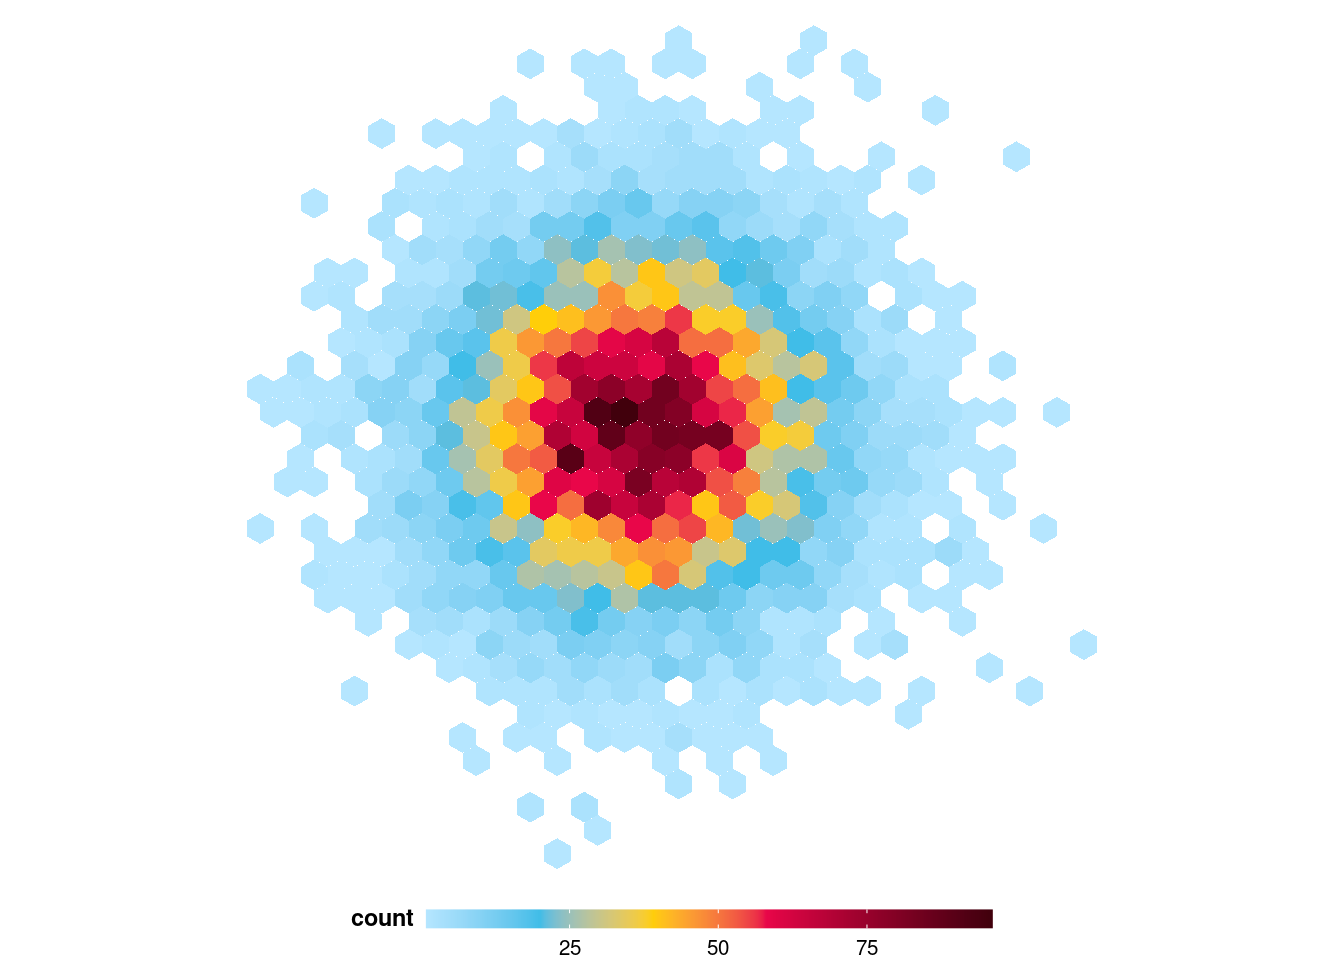
\includegraphics[height=0.5\textheight]{figures/continous_palette-1} \end{center}

\hypertarget{theme}{%
\section{Theme}\label{theme}}

The major goal of the theme was to keep things simple so that you could concentrate
on the data. As a result, the chart's components, such as the axes, are smaller and less eye - catching.

\begin{Shaded}
\begin{Highlighting}[]
\NormalTok{k }\OtherTok{=} \DecValTok{5}
\NormalTok{df1 }\OtherTok{=} \FunctionTok{data.frame}\NormalTok{(}\AttributeTok{x =} \FunctionTok{rnorm}\NormalTok{(}\DecValTok{100}\SpecialCharTok{*}\NormalTok{k), }\AttributeTok{y =} \FunctionTok{rnorm}\NormalTok{(}\DecValTok{100}\SpecialCharTok{*}\NormalTok{k),}\AttributeTok{type =}\NormalTok{ letters[}\DecValTok{1}\SpecialCharTok{:}\NormalTok{k]) }\SpecialCharTok{\%\textgreater{}\%} 
  \FunctionTok{mutate}\NormalTok{(}\AttributeTok{x =}\NormalTok{ x}\SpecialCharTok{+} \FunctionTok{as.integer}\NormalTok{(}\FunctionTok{as.factor}\NormalTok{(type)))}
\FunctionTok{ggplot}\NormalTok{(df1,}\FunctionTok{aes}\NormalTok{(}\AttributeTok{x =}\NormalTok{ x, }\AttributeTok{fill =}\NormalTok{ type)) }\SpecialCharTok{+} 
  \FunctionTok{geom\_density}\NormalTok{(}\AttributeTok{col =} \StringTok{"transparent"}\NormalTok{,}\AttributeTok{alpha =} \FloatTok{0.7}\NormalTok{) }\SpecialCharTok{+} 
  \FunctionTok{labs}\NormalTok{(}\AttributeTok{x =} \StringTok{"X Value"}\NormalTok{,}\AttributeTok{y =} \StringTok{"Density"}\NormalTok{)}\SpecialCharTok{+}
  \FunctionTok{bottom\_legend}\NormalTok{()}
\end{Highlighting}
\end{Shaded}

\begin{center}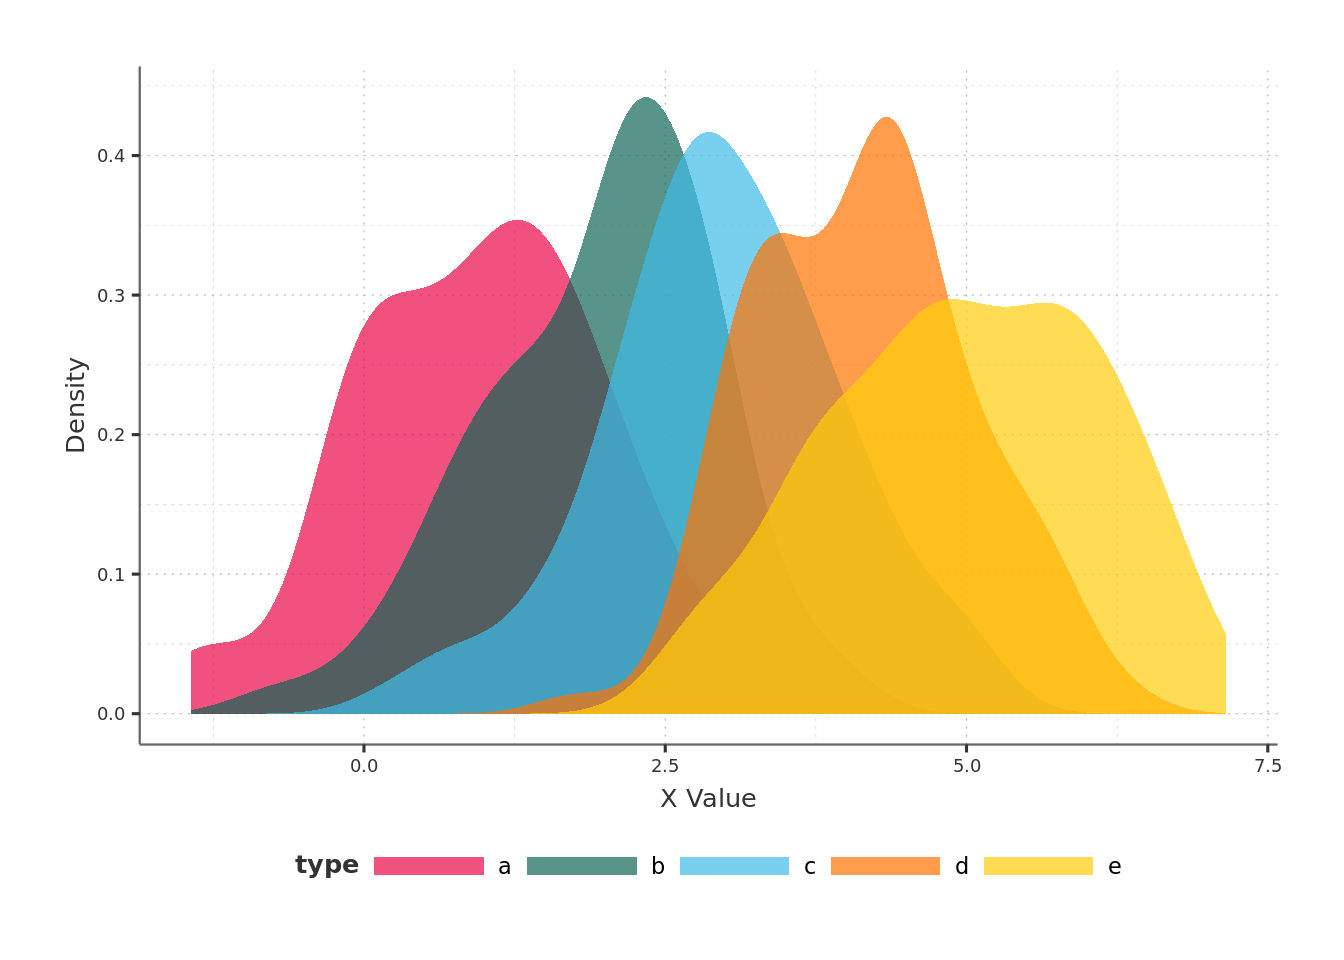
\includegraphics{figures/mpithemes_theme_scientific-1} \end{center}

\hypertarget{table-1}{%
\chapter{Table}\label{table-1}}

In data analysis, providing a summary of the data in the form of a table, in addition to generating a graph, is highly beneficial for expressing the results.

To generate tables, you can use a variety of R packages.
\href{https://haozhu233.github.io/kableExtra/}{kableExtra} and \href{https://gt.rstudio.com/}{gt} are the two main packages

\hypertarget{gt}{%
\section{gt}\label{gt}}

To learn about the gt package features and see many examples, you can see
An informative document, \href{https://themockup.blog/static/gt-cookbook.html\#Introduction}{gt-cookbook}.

\begin{Shaded}
\begin{Highlighting}[]
\FunctionTok{head}\NormalTok{(mtcars) }\SpecialCharTok{\%\textgreater{}\%} 
  \FunctionTok{gt}\NormalTok{(}\AttributeTok{rownames\_to\_stub =} \ConstantTok{TRUE}\NormalTok{) }\SpecialCharTok{\%\textgreater{}\%} 
  \FunctionTok{opt\_row\_striping}\NormalTok{() }\SpecialCharTok{\%\textgreater{}\%} 
  \FunctionTok{tab\_header}\NormalTok{(}
    \AttributeTok{title =} \StringTok{"Motor Trend Car Road Tests"}\NormalTok{,}
    \AttributeTok{subtitle =} \StringTok{"From the 1974 Motor Trend US magazine"}
\NormalTok{  )}
\end{Highlighting}
\end{Shaded}

\captionsetup[table]{labelformat=empty,skip=1pt}
\begin{longtable}{lrrrrrrrrrrr}
\caption*{
{\large Motor Trend Car Road Tests} \\ 
{\small From the 1974 Motor Trend US magazine}
} \\ 
\toprule
 & mpg & cyl & disp & hp & drat & wt & qsec & vs & am & gear & carb \\ 
\midrule
Mazda RX4 & 21.0 & 6 & 160 & 110 & 3.90 & 2.620 & 16.46 & 0 & 1 & 4 & 4 \\ 
Mazda RX4 Wag & 21.0 & 6 & 160 & 110 & 3.90 & 2.875 & 17.02 & 0 & 1 & 4 & 4 \\ 
Datsun 710 & 22.8 & 4 & 108 & 93 & 3.85 & 2.320 & 18.61 & 1 & 1 & 4 & 1 \\ 
Hornet 4 Drive & 21.4 & 6 & 258 & 110 & 3.08 & 3.215 & 19.44 & 1 & 0 & 3 & 1 \\ 
Hornet Sportabout & 18.7 & 8 & 360 & 175 & 3.15 & 3.440 & 17.02 & 0 & 0 & 3 & 2 \\ 
Valiant & 18.1 & 6 & 225 & 105 & 2.76 & 3.460 & 20.22 & 1 & 0 & 3 & 1 \\ 
 \bottomrule
\end{longtable}

Many features of the \texttt{gt} package can be customized, including:

\begin{itemize}
\tightlist
\item
  Make changes to the table columns format, color, size and\ldots{}
\item
  Insert row information, including names and groups.
\item
  Use headers, spanners, and footers to add extra information.
\item
  Change table style.
\end{itemize}

\begin{Shaded}
\begin{Highlighting}[]
\NormalTok{gtcars }\SpecialCharTok{\%\textgreater{}\%}
    \FunctionTok{filter}\NormalTok{(ctry\_origin }\SpecialCharTok{\%in\%} \FunctionTok{c}\NormalTok{(}\StringTok{"United States"}\NormalTok{, }\StringTok{"Japan"}\NormalTok{)) }\SpecialCharTok{\%\textgreater{}\%}
    \FunctionTok{select}\NormalTok{(mfr}\SpecialCharTok{:}\NormalTok{year, mpg\_c, mpg\_h, ctry\_origin, msrp) }\SpecialCharTok{\%\textgreater{}\%} 
    \FunctionTok{gt}\NormalTok{(}
        \AttributeTok{rowname\_col =} \StringTok{"ctry\_origin"}\NormalTok{,}
        \AttributeTok{groupname\_col =} \StringTok{"year"}
\NormalTok{    ) }\SpecialCharTok{\%\textgreater{}\%}
    \FunctionTok{summary\_rows}\NormalTok{(}
        \AttributeTok{groups =} \ConstantTok{TRUE}\NormalTok{,}
        \AttributeTok{columns =} \FunctionTok{c}\NormalTok{(}\StringTok{"msrp"}\NormalTok{),}
        \AttributeTok{fns =} \FunctionTok{list}\NormalTok{(}\AttributeTok{Total =} \SpecialCharTok{\textasciitilde{}}\FunctionTok{sum}\NormalTok{(.))}
\NormalTok{    ) }\SpecialCharTok{\%\textgreater{}\%}
    \FunctionTok{grand\_summary\_rows}\NormalTok{(}
        \AttributeTok{columns =} \FunctionTok{c}\NormalTok{(}\StringTok{"msrp"}\NormalTok{),}
        \AttributeTok{fns =} \FunctionTok{list}\NormalTok{(}\AttributeTok{Overall =} \SpecialCharTok{\textasciitilde{}}\FunctionTok{sum}\NormalTok{(.))}
\NormalTok{    ) }\SpecialCharTok{\%\textgreater{}\%} 
  \FunctionTok{data\_color}\NormalTok{(}
    \AttributeTok{columns =} \FunctionTok{c}\NormalTok{(}\StringTok{"mpg\_c"}\NormalTok{, }\StringTok{"mpg\_h"}\NormalTok{),}
    \AttributeTok{colors =}\NormalTok{ scales}\SpecialCharTok{::}\FunctionTok{col\_numeric}\NormalTok{(}
      \AttributeTok{palette =} \FunctionTok{c}\NormalTok{(}
        \StringTok{"white"}\NormalTok{, }\StringTok{"green"}\NormalTok{),}
      \AttributeTok{domain =} \FunctionTok{c}\NormalTok{(}\DecValTok{10}\NormalTok{, }\DecValTok{25}\NormalTok{))}
\NormalTok{  ) }\SpecialCharTok{\%\textgreater{}\%} 
  \FunctionTok{fmt\_missing}\NormalTok{(}
        \AttributeTok{columns =} \FunctionTok{contains}\NormalTok{(}\StringTok{"mpg"}\NormalTok{),}
        \AttributeTok{missing\_text =} \StringTok{""}
\NormalTok{    )}
\end{Highlighting}
\end{Shaded}

\captionsetup[table]{labelformat=empty,skip=1pt}
\begin{longtable}{lllrrr}
\toprule
 & mfr & model & mpg\_c & mpg\_h & msrp \\ 
\midrule
\multicolumn{1}{l}{2017} \\ 
\midrule
United States & Ford & GT & 11 & 18 & 447000 \\ 
Japan & Acura & NSX & 21 & 22 & 156000 \\ 
United States & Dodge & Viper & 12 & 19 & 95895 \\ 
United States & Tesla & Model S &  &  & 74500 \\ 
\midrule 
Total & — & — & — & — & $773,395.00$ \\ 
\midrule
\multicolumn{1}{l}{2016} \\ 
\midrule
Japan & Nissan & GT-R & 16 & 22 & 101770 \\ 
United States & Chevrolet & Corvette & 15 & 22 & 88345 \\ 
\midrule 
Total & — & — & — & — & $190,115.00$ \\ 
 \midrule 
\midrule 
Overall & — & — & — & — & $963,510.00$ \\ 
\bottomrule
\end{longtable}

\hypertarget{kableextra}{%
\section{kableExtra}\label{kableextra}}

The \texttt{kableExtra} package is intended to enhance the basic functionality of \texttt{knitr::kable} tables.
The most impressive aspect of \texttt{kableExtra} is that the majority of its table capabilities are compatible with both HTML and PDF. It's a good choice of \texttt{kableExtra} if you can generate a PDF (LaTex) report. For more example of use this package for PDF output see this
\href{http://haozhu233.github.io/kableExtra/awesome_table_in_pdf.pdf}{manual}.
Below, there are some examples from kableExtra documents that are shown.
strongly recommends using the \texttt{booktabs\ =\ T} option for pdf output.
In the HTML manual, this option is removed.

\begin{Shaded}
\begin{Highlighting}[]
\NormalTok{dt }\OtherTok{\textless{}{-}}\NormalTok{ mtcars[}\DecValTok{1}\SpecialCharTok{:}\DecValTok{5}\NormalTok{, }\DecValTok{1}\SpecialCharTok{:}\DecValTok{6}\NormalTok{]}
\NormalTok{dt }\SpecialCharTok{\%\textgreater{}\%} 
\FunctionTok{kbl}\NormalTok{() }\SpecialCharTok{\%\textgreater{}\%}
    \FunctionTok{kable\_material}\NormalTok{(}\FunctionTok{c}\NormalTok{(}\StringTok{"striped"}\NormalTok{, }\StringTok{"hover"}\NormalTok{))}
\end{Highlighting}
\end{Shaded}

\begin{table}
\centering
\begin{tabular}[t]{l|r|r|r|r|r|r}
\hline
  & mpg & cyl & disp & hp & drat & wt\\
\hline
Mazda RX4 & 21.0 & 6 & 160 & 110 & 3.90 & 2.620\\
\hline
Mazda RX4 Wag & 21.0 & 6 & 160 & 110 & 3.90 & 2.875\\
\hline
Datsun 710 & 22.8 & 4 & 108 & 93 & 3.85 & 2.320\\
\hline
Hornet 4 Drive & 21.4 & 6 & 258 & 110 & 3.08 & 3.215\\
\hline
Hornet Sportabout & 18.7 & 8 & 360 & 175 & 3.15 & 3.440\\
\hline
\end{tabular}
\end{table}

\begin{Shaded}
\begin{Highlighting}[]
\NormalTok{mtcars[}\DecValTok{1}\SpecialCharTok{:}\DecValTok{8}\NormalTok{, }\DecValTok{1}\SpecialCharTok{:}\DecValTok{8}\NormalTok{] }\SpecialCharTok{\%\textgreater{}\%}
  \FunctionTok{kbl}\NormalTok{() }\SpecialCharTok{\%\textgreater{}\%}
  \FunctionTok{kable\_paper}\NormalTok{(}\AttributeTok{full\_width =}\NormalTok{ F) }\SpecialCharTok{\%\textgreater{}\%}
  \FunctionTok{column\_spec}\NormalTok{(}\DecValTok{2}\NormalTok{, }\AttributeTok{color =} \FunctionTok{spec\_color}\NormalTok{(mtcars}\SpecialCharTok{$}\NormalTok{mpg[}\DecValTok{1}\SpecialCharTok{:}\DecValTok{8}\NormalTok{]),}
              \AttributeTok{link =} \StringTok{"https://haozhu233.github.io/kableExtra/"}\NormalTok{) }\SpecialCharTok{\%\textgreater{}\%}
  \FunctionTok{column\_spec}\NormalTok{(}\DecValTok{6}\NormalTok{, }\AttributeTok{color =} \StringTok{"white"}\NormalTok{,}
              \AttributeTok{background =} \FunctionTok{spec\_color}\NormalTok{(mtcars}\SpecialCharTok{$}\NormalTok{drat[}\DecValTok{1}\SpecialCharTok{:}\DecValTok{8}\NormalTok{], }\AttributeTok{end =} \FloatTok{0.7}\NormalTok{),}
              \AttributeTok{popover =} \FunctionTok{paste}\NormalTok{(}\StringTok{"am:"}\NormalTok{, mtcars}\SpecialCharTok{$}\NormalTok{am[}\DecValTok{1}\SpecialCharTok{:}\DecValTok{8}\NormalTok{]))}
\end{Highlighting}
\end{Shaded}

\begin{table}
\centering
\begin{tabular}[t]{l|>{}r|r|r|r|>{}r|r|r|r}
\hline
  & mpg & cyl & disp & hp & drat & wt & qsec & vs\\
\hline
Mazda RX4 & \href{https://haozhu233.github.io/kableExtra/}{\textcolor[HTML]{34B679}{21.0}} & 6 & 160.0 & 110 & \cellcolor[HTML]{43BF71}{\textcolor{white}{3.90}} & 2.620 & 16.46 & 0\\
\hline
Mazda RX4 Wag & \href{https://haozhu233.github.io/kableExtra/}{\textcolor[HTML]{34B679}{21.0}} & 6 & 160.0 & 110 & \cellcolor[HTML]{43BF71}{\textcolor{white}{3.90}} & 2.875 & 17.02 & 0\\
\hline
Datsun 710 & \href{https://haozhu233.github.io/kableExtra/}{\textcolor[HTML]{95D840}{22.8}} & 4 & 108.0 & 93 & \cellcolor[HTML]{37B878}{\textcolor{white}{3.85}} & 2.320 & 18.61 & 1\\
\hline
Hornet 4 Drive & \href{https://haozhu233.github.io/kableExtra/}{\textcolor[HTML]{44BF70}{21.4}} & 6 & 258.0 & 110 & \cellcolor[HTML]{414387}{\textcolor{white}{3.08}} & 3.215 & 19.44 & 1\\
\hline
Hornet Sportabout & \href{https://haozhu233.github.io/kableExtra/}{\textcolor[HTML]{26818E}{18.7}} & 8 & 360.0 & 175 & \cellcolor[HTML]{3C4F8A}{\textcolor{white}{3.15}} & 3.440 & 17.02 & 0\\
\hline
Valiant & \href{https://haozhu233.github.io/kableExtra/}{\textcolor[HTML]{2C728E}{18.1}} & 6 & 225.0 & 105 & \cellcolor[HTML]{440154}{\textcolor{white}{2.76}} & 3.460 & 20.22 & 1\\
\hline
Duster 360 & \href{https://haozhu233.github.io/kableExtra/}{\textcolor[HTML]{440154}{14.3}} & 8 & 360.0 & 245 & \cellcolor[HTML]{375A8C}{\textcolor{white}{3.21}} & 3.570 & 15.84 & 0\\
\hline
Merc 240D & \href{https://haozhu233.github.io/kableExtra/}{\textcolor[HTML]{FDE725}{24.4}} & 4 & 146.7 & 62 & \cellcolor[HTML]{1FA187}{\textcolor{white}{3.69}} & 3.190 & 20.00 & 1\\
\hline
\end{tabular}
\end{table}

\begin{Shaded}
\begin{Highlighting}[]
\NormalTok{mpg\_list }\OtherTok{\textless{}{-}} \FunctionTok{split}\NormalTok{(mtcars}\SpecialCharTok{$}\NormalTok{mpg, mtcars}\SpecialCharTok{$}\NormalTok{cyl)}
\NormalTok{disp\_list }\OtherTok{\textless{}{-}} \FunctionTok{split}\NormalTok{(mtcars}\SpecialCharTok{$}\NormalTok{disp, mtcars}\SpecialCharTok{$}\NormalTok{cyl)}
\NormalTok{inline\_plot }\OtherTok{\textless{}{-}} \FunctionTok{data.frame}\NormalTok{(}\AttributeTok{cyl =} \FunctionTok{c}\NormalTok{(}\DecValTok{4}\NormalTok{, }\DecValTok{6}\NormalTok{, }\DecValTok{8}\NormalTok{), }\AttributeTok{mpg\_box =} \StringTok{""}\NormalTok{, }\AttributeTok{mpg\_hist =} \StringTok{""}\NormalTok{,}
                          \AttributeTok{mpg\_line1 =} \StringTok{""}\NormalTok{, }\AttributeTok{mpg\_line2 =} \StringTok{""}\NormalTok{,}
                          \AttributeTok{mpg\_points1 =} \StringTok{""}\NormalTok{, }\AttributeTok{mpg\_points2 =} \StringTok{""}\NormalTok{, }\AttributeTok{mpg\_poly =} \StringTok{""}\NormalTok{)}
\NormalTok{inline\_plot }\SpecialCharTok{\%\textgreater{}\%}
  \FunctionTok{kbl}\NormalTok{(}\AttributeTok{booktabs =} \ConstantTok{TRUE}\NormalTok{) }\SpecialCharTok{\%\textgreater{}\%}
  \FunctionTok{kable\_paper}\NormalTok{(}\AttributeTok{full\_width =} \ConstantTok{FALSE}\NormalTok{) }\SpecialCharTok{\%\textgreater{}\%}
  \FunctionTok{column\_spec}\NormalTok{(}\DecValTok{2}\NormalTok{, }\AttributeTok{image =} \FunctionTok{spec\_boxplot}\NormalTok{(mpg\_list)) }\SpecialCharTok{\%\textgreater{}\%}
  \FunctionTok{column\_spec}\NormalTok{(}\DecValTok{3}\NormalTok{, }\AttributeTok{image =} \FunctionTok{spec\_hist}\NormalTok{(mpg\_list)) }\SpecialCharTok{\%\textgreater{}\%}
  \FunctionTok{column\_spec}\NormalTok{(}\DecValTok{4}\NormalTok{, }\AttributeTok{image =} \FunctionTok{spec\_plot}\NormalTok{(mpg\_list, }\AttributeTok{same\_lim =} \ConstantTok{TRUE}\NormalTok{)) }\SpecialCharTok{\%\textgreater{}\%}
  \FunctionTok{column\_spec}\NormalTok{(}\DecValTok{5}\NormalTok{, }\AttributeTok{image =} \FunctionTok{spec\_plot}\NormalTok{(mpg\_list, }\AttributeTok{same\_lim =} \ConstantTok{FALSE}\NormalTok{)) }\SpecialCharTok{\%\textgreater{}\%}
  \FunctionTok{column\_spec}\NormalTok{(}\DecValTok{6}\NormalTok{, }\AttributeTok{image =} \FunctionTok{spec\_plot}\NormalTok{(mpg\_list, }\AttributeTok{type =} \StringTok{"p"}\NormalTok{)) }\SpecialCharTok{\%\textgreater{}\%}
  \FunctionTok{column\_spec}\NormalTok{(}\DecValTok{7}\NormalTok{, }\AttributeTok{image =} \FunctionTok{spec\_plot}\NormalTok{(mpg\_list, disp\_list, }\AttributeTok{type =} \StringTok{"p"}\NormalTok{)) }\SpecialCharTok{\%\textgreater{}\%}
  \FunctionTok{column\_spec}\NormalTok{(}\DecValTok{8}\NormalTok{, }\AttributeTok{image =} \FunctionTok{spec\_plot}\NormalTok{(mpg\_list, }\AttributeTok{polymin =} \DecValTok{5}\NormalTok{))}
\end{Highlighting}
\end{Shaded}

\begin{table}
\centering
\begin{tabular}[t]{r>{}l>{}l>{}l>{}l>{}l>{}l>{}l}
\toprule
cyl & mpg\_box & mpg\_hist & mpg\_line1 & mpg\_line2 & mpg\_points1 & mpg\_points2 & mpg\_poly\\
\midrule
4 & 
\includegraphics[width=0.67in, height=0.17in]{estimation-graphical-model_2_files/figure-latex//boxplot_5672ab2c1708.pdf} & 
\includegraphics[width=0.67in, height=0.17in]{estimation-graphical-model_2_files/figure-latex//hist_5672a77e1f3e3.pdf} & 
\includegraphics[width=0.67in, height=0.17in]{estimation-graphical-model_2_files/figure-latex//plot_5672a76ebb0f7.pdf} & 
\includegraphics[width=0.67in, height=0.17in]{estimation-graphical-model_2_files/figure-latex//plot_5672a5c7f739b.pdf} & 
\includegraphics[width=0.67in, height=0.17in]{estimation-graphical-model_2_files/figure-latex//plot_5672a6a2c6ae8.pdf} & 
\includegraphics[width=0.67in, height=0.17in]{estimation-graphical-model_2_files/figure-latex//plot_5672a55f901b.pdf} & 
\includegraphics[width=0.67in, height=0.17in]{estimation-graphical-model_2_files/figure-latex//plot_5672a47ef4457.pdf}\\
6 & 
\includegraphics[width=0.67in, height=0.17in]{estimation-graphical-model_2_files/figure-latex//boxplot_5672a7a439b5b.pdf} & 
\includegraphics[width=0.67in, height=0.17in]{estimation-graphical-model_2_files/figure-latex//hist_5672a698f1ddf.pdf} & 
\includegraphics[width=0.67in, height=0.17in]{estimation-graphical-model_2_files/figure-latex//plot_5672a3baab6ef.pdf} & 
\includegraphics[width=0.67in, height=0.17in]{estimation-graphical-model_2_files/figure-latex//plot_5672a58c6c23a.pdf} & 
\includegraphics[width=0.67in, height=0.17in]{estimation-graphical-model_2_files/figure-latex//plot_5672a48658f6c.pdf} & 
\includegraphics[width=0.67in, height=0.17in]{estimation-graphical-model_2_files/figure-latex//plot_5672a11a97f9f.pdf} & 
\includegraphics[width=0.67in, height=0.17in]{estimation-graphical-model_2_files/figure-latex//plot_5672a578f0dd1.pdf}\\
8 & 
\includegraphics[width=0.67in, height=0.17in]{estimation-graphical-model_2_files/figure-latex//boxplot_5672a3a7b7d30.pdf} & 
\includegraphics[width=0.67in, height=0.17in]{estimation-graphical-model_2_files/figure-latex//hist_5672aaba160d.pdf} & 
\includegraphics[width=0.67in, height=0.17in]{estimation-graphical-model_2_files/figure-latex//plot_5672a5bfc678.pdf} & 
\includegraphics[width=0.67in, height=0.17in]{estimation-graphical-model_2_files/figure-latex//plot_5672a2e4895af.pdf} & 
\includegraphics[width=0.67in, height=0.17in]{estimation-graphical-model_2_files/figure-latex//plot_5672a614fd349.pdf} & 
\includegraphics[width=0.67in, height=0.17in]{estimation-graphical-model_2_files/figure-latex//plot_5672a101123cb.pdf} & 
\includegraphics[width=0.67in, height=0.17in]{estimation-graphical-model_2_files/figure-latex//plot_5672a5ee8418b.pdf}\\
\bottomrule
\end{tabular}
\end{table}

\hypertarget{environment}{%
\chapter{Environment}\label{environment}}

Block content can be useful for informing or alerting your readers about a specific topic.
We use the \texttt{awesomebox} and \texttt{tcolorbox} Latex packages for colored block content.
For supplemental information, you can use notes, tips, info, error, and warning elements. Each block serves a specific semantic purpose.

\begin{rmdNote}
Lorem Ipsum is simply dummy text of the printing and typesetting industry.

\end{rmdNote}

\begin{rmdnote}
Lorem Ipsum is simply dummy text of the printing and typesetting industry.

\end{rmdnote}

\begin{rmdTip}
Lorem Ipsum is simply dummy text of the printing and typesetting industry.

\end{rmdTip}

\begin{rmdtip}
Lorem Ipsum is simply dummy text of the printing and typesetting industry.

\end{rmdtip}

\begin{rmdThink}
Lorem Ipsum is simply dummy text of the printing and typesetting industry.

\end{rmdThink}

\begin{rmdthink}
Lorem Ipsum is simply dummy text of the printing and typesetting industry.

\end{rmdthink}

\begin{rmdWarning}
Lorem Ipsum is simply dummy text of the printing and typesetting industry.

\end{rmdWarning}

\begin{rmdwarning}
Lorem Ipsum is simply dummy text of the printing and typesetting industry.

\end{rmdwarning}

\begin{rmdTodo}
Lorem Ipsum is simply dummy text of the printing and typesetting industry.

\end{rmdTodo}

\begin{rmdtodo}
Lorem Ipsum is simply dummy text of the printing and typesetting industry.

\end{rmdtodo}

\begin{Theorem}{}{}
Lorem Ipsum is simply dummy text of the printing and typesetting industry.

\end{Theorem}

\begin{Definition}{}{}
Lorem Ipsum is simply dummy text of the printing and typesetting industry.

\end{Definition}

\begin{Lemma}{}{}
Lorem Ipsum is simply dummy text of the printing and typesetting industry.

\end{Lemma}

\begin{Corollary}{}{}
Lorem Ipsum is simply dummy text of the printing and typesetting industry.

\end{Corollary}

\begin{Proposition}{}{}
Lorem Ipsum is simply dummy text of the printing and typesetting industry.

\end{Proposition}

\begin{Exercise}{}{}
Lorem Ipsum is simply dummy text of the printing and typesetting industry.

\end{Exercise}

\begin{Example}{}{}
Lorem Ipsum is simply dummy text of the printing and typesetting industry.

\end{Example}

\begin{Remark}{}{}
Lorem Ipsum is simply dummy text of the printing and typesetting industry.

\end{Remark}

\begin{Proof}{}{}
Lorem Ipsum is simply dummy text of the printing and typesetting industry.

\end{Proof}

\begin{Solution}{}{}
Lorem Ipsum is simply dummy text of the printing and typesetting industry.

\end{Solution}

\begin{rmdexer}
Lorem Ipsum is simply dummy text of the printing and typesetting industry.

\end{rmdexer}

\begin{rmdsol}
Lorem Ipsum is simply dummy text of the printing and typesetting industry.

\end{rmdsol}

\hypertarget{reference}{%
\chapter{Reference}\label{reference}}



\end{document}
